\documentclass[a4paper, 12pt, oneside]{extarticle}
\input{$UNI/.templates/settings/preamble}
%shell-escape
\input{$UNI/.templates/settings/minted_settings.tex}
\usepackage{etoolbox} % пакунок для розширеного програмування
\usepackage{enumerate} % пакунок для розширеного програмування

\newtoggle{Report}
\togglefalse{Report}

\newtoggle{ShowVar}
\toggletrue{ShowVar} % якщо true, то відображається варіант замість теми
\renewcommand\Department{ОМП}

\newcommand\Type{\RGR}
\newcommand\Number{1}
\newcommand\Discipline{Теорія ймовірностей та математична статистика}
\newcommand\Topic{TOPIC}

\newcommand\Class{студент групи \Group}
\newcommand\Author{\Lname~\Initials}
\newcommand\Position{доцент}
\newcommand\Instructor{Білущак Г. І.}
\renewcommand\Variant{14}

\usepackage{pgfplots}
\pgfplotsset{compat=1.17}

\usepackage{boxedminipage}
\usepackage{varwidth}
\fboxrule=1pt

\usepackage{titlesec, blindtext, color}
\definecolor{gray75}{gray}{0.75}
\newcommand{\hsp}{\hspace{10pt}}
\titleformat{\chapter}[hang]{\Huge\bfseries}{\thechapter\hsp\textcolor{gray75}{|}\hsp}{0pt}{\Huge\bfseries}


\renewcommand{\thesubsection}{\arabic{subsection}}

\titleformat{\subsection}[hang]{\normalsize\bfseries}{\thesubsection{.}\hsp}{0pt}{\normalsize\normalfont}

% \usepackage{macrolist}
% \macronewlist{Answers}

% ЗАВДАННЯ
\newcommand{\Problem}{\subsection}
% РОЗВ'ЯЗОК
\newcommand{\Solution}{\subsubsection*{\centering \scshape Розв'язок:}}
% ВІДПОВІДЬ
\newcommand{\Answer}[1]{
\medskip
\null\hfill
\begin{boxedminipage}{\textwidth}
	\paragraph{Відповідь: }{#1}
	% \macrolistadd{Answers}{#1}
\end{boxedminipage}
}

\usetikzlibrary{patterns}

\begin{document}

\newgeometry{top=1cm,bottom=1cm,right=1.5cm,left=1.5cm}
\newcommand{\LINE}{\rule{\linewidth}{0.4mm}}
\begin{titlepage}
	\center

	\textsc{МІНІСТЕРСТВО ОСВІТИ І НАУКИ УКРАЇНИ}\\
	\textsc{НАЦІОНАЛЬНИЙ УНІВЕРСИТЕТ "`ЛЬВІВСЬКА ПОЛІТЕХНІКА"'}\\
	% \textsc{національний університет ``львівська політехніка''}\\
	\small
	\iftoggle{RGR} {}
	{
		{\Institute}\\
	}
	{кафедра \Department}\\
	[1.5cm]
	\normalsize
	%\large

	\includegraphics[scale=0.35]{$HOME/Templates/lpnu_doc_templates/lpnu_logo.png}\\[1.5cm]

	\iftoggle{Report}
	{
		\textsc{\LARGE\bfseries звіт}\\
		\textsc{ до \Type \, \No\Number}\\
	}
	{
		\textsc{\LARGE\bfseries \Type~\Number}\\
	}
до розрахунково-графічної роботи \\
  з дисципліни: "`\Discipline"'\\
  %на тему: \\

	\iftoggle{RGR}
	{
	\LINE\\[0.2cm] % норм?
	\large
		\textsc{\bfseries Варіант \Variant}\\[0cm]
	\LINE\\[1cm]
	}
	{
	\LINE\\[0.2cm]
	\large
	\textsc{\bfseries \Topic}\\[0cm]
	\normalsize
	\LINE\\[1cm]
	}


	\begin{flushright}
		\large
		\textit{Виконав}\\
		\normalsize
		\Class \; \textsc{\Author}

		\large
		\textit{Перевірив(ла)}\\
		\normalsize
		\Position \; \textsc{\Instructor}
	\end{flushright}

	\vfill
	Львів	\the\year{}
\end{titlepage}
\Margins


\Problem{Скількома способами можна 10 різних олівців
розкласти у три пенали?}

Перші 3 олівці можна розкласти 6 способами, а далі кожен
можна в 1 із 3 пеналів.

$
6*3^7
= 13122
$
.

\Answer{13122}

\Problem{Гральна кістка підкидається один раз. Результат експерименту --- число очок на верхній грані. Розглянемо події: $M$ --- випала четвірка; $N$ --- випало менше, ніж 3 очки; $K$ --- випала непарна кількість очок. Які з даних подій сумісні, а які --- ні? Описати події: $M \cap N, N \cap K, M \cup N, N \cup K, \bar N, \bar K, M \cup N \cup K, M \cap N \cap K$.}

$$
m=4, n<3, k\%2=1
$$

Сумісні $N$ і $K$. Більше нема сумісних.

$$
\begin{array}{ll}
	M \cap N = \emptyset &
	N \cap K = 1 \\
	M \cup N = \{4, 2, 1\} &
	N \cup K = \{1,2,3,5\} \\
	% \not N о кльово
	\bar N = \{3,4,5,6\} &
	\bar K = \{2,4,6\} \\
	M \cup N \cup K = \{4,1,2,3,5\} &
	M \cap N \cap K = \emptyset
\end{array}
$$

\Problem{З набору доміно (28 штук) навмання виймають 7 кісток. Яка ймовірність того, що серед них виявиться: а) саме 2 ``дублі''; б) жодного ``дубля''?}

способів вибрати 7 кісток із 28:

$$
	\frac{28!}{(28-7)!7!} = C_{28}^7
$$

\begin{enumerate}[a)]
	\item саме 2 дублі:
		$
			\frac{C_7^2 \cdot C_{21}^5}{C_{28}^7}
		$

\begin{minted}{r}
> c_7_28 = factorial(28)/(factorial(28-7)*factorial(7))
> c_2_7 = factorial(7)/(factorial(5)*factorial(2))
> c_5_21 = factorial(21)/(factorial(21-5)*factorial(5))
> c_2_7 * c_5_21 / c_7_28
[1] 0.3609076
\end{minted}

	\item жодного дубля
		$
			\frac{C_7^0 \cdot C_{21}^7}{C_{28}^7}
		$
\begin{minted}{r}
> c_0_7*c_7_21/c_7_28
[1] 0.09820614
\end{minted}

\end{enumerate}

\Answer{
	а) 0.3609076;
	б) 0.09820614
}

\Problem{
	Усередині квадрата зі стороною 8 см навмання вибрана точка. Яка ймовірність того, що віддаль від неї до фіксованої сторони не перевищуватиме 6 см ?
}

\begin{figure}[h]
	\centering
\begin{tikzpicture}
    % Малюємо квадрат
    \draw (0,0) rectangle (2,2);
    % Додаємо позначення
    \node at (1, 2.25) {8 см};
    % Заштриховуємо внутрішню площу
    \fill[pattern=north west lines] (0,0) rectangle (1.5,2);
\end{tikzpicture}
	\caption{квадрат}
	\label{kvadrat}
\end{figure}

На рис. \ref{kvadrat} зображений заданий квадрат. Заштрихована площа відображає розташування точки відносно фіксованої сторони, яке задовольняє умову.
Вона дорівнює $6 \cdot 8 = 48$ см. Отримуємо таку ймовірність: $\frac{48}{64} = \frac{3}{4}$

\Answer{
	$\frac{3}{4}$
}

\Problem{
	Проводяться три незалежні постріли снарядами з імовірністю влучання 0.6 кожен. Ціль знищується з імовірністю 0.5 при влучанні одним снарядом, з імовірністю 0.9 двома та з імовірністю 1 після влучання трьома снарядами. а) Знайти ймовірність знищення цілі; б) Нехай ціль знищена. Яка ймовірність того, що в неї влучив тільки один снаряд?
}
% комніьації?
\begin{enumerate}[a)]
	\item Імовірності попадання
		\begin{itemize}
			\item один раз:
				$
					C_3^1 * 0.6 * 0.4^2 = 3 * 0.6 * 0.4^2 = 0.288
				$
			\item два рази:
				$
					C_3^2 * 0.6^2 * 0.4 = 3 * 0.6^2 * 0.4 = 0.432
				$
			\item три рази:
				$
					C_3^3 * 0.6^3 = 0.216
				$
		\end{itemize}
		Імовірність знищення цілі:
		$
		0.288 * 0.5 + 0.432 * 0.9 + 0.216 * 1
		= 0.7488
		$ % так треба тут імовірності незнищення чи нє? <++>
	\item Імовірність влучання тільки одного снаряду, коли ціль знищена:

		Формула Баєса:
		$$
		P_A(B_1) = \frac{P(B_1)P_{B_1}(A)}{P(A)}
		= \frac{0.288 * 0.288 * 0.5}{0.7488}
		\approx 0.05537869885695972652
		$$
% Тепер, коли ціль знищена, ймовірність того, що в неї влучив тільки один снаряд, дорівнює нулю, оскільки ціль була знищена. Нема сенсу стріляти по знищеній цілі.

\end{enumerate}

\Answer{Імовірність знищення цілі --- 0.7488,

ймовірність влучання тільки одного снаряду за умови знищення: 0.0553.}

\Problem{
	Підкидаємо гральну кістку. Що ймовірніше: з 6 підкидань число 5 випаде саме 2 рази чи з 3 підкидань число 2 випаде саме один раз?
}

За схемою Бернуллі маємо:

$$
P_1 =
C_6^2
\cdot
\frac{1^2}{6^2}
\cdot
\frac{5^4}{6^4}
% \approx 15 \cdot 0.01
\approx 0.15
$$

% $$
% P(A) = \frac{C_{30}^{3}}{C_{45}^{5}} =\frac{\frac{30!}{3! \cdot 27!}}{\frac{45!}{5! \cdot 40!}}
% =\frac{\frac{30 \cdot 29 \cdot 28}{3 \cdot 2 \cdot 1}}{\frac{45 \cdot 44 \cdot 43 \cdot 42 \cdot 41 \cdot 40}{5 \cdot 4 \cdot 3 \cdot 2 \cdot 1}}
% =\frac{4060}{122175} = 0.0332
% P(B) = /frac{C_{30}^{4}}{C_{45}^{5}}
% P(C)
% $$

$$
P_2 =
C_3^1
\cdot
\frac{1}{6}
\cdot
\frac{5^2}{6^2}
\approx 0.3
$$


\Answer{Імовірніше те, що з 3 підкидань 1 раз випаде число 2.}

\Problem{
	Знайти закон розподілу дискретної випадкової величини $\xi$, яка може набувати лише двох значень: $x_1$ з імовірністю
	$p_1=0.3$ і
	$x_2$, якщо $x_1<x_2$ і
	$M\xi=3.1, D\xi=1.89$.
}

$$
M(X) = x_1p_1 + \cdots + x_n p_n,\,
% /home/sasha/Documents/uni/statistics/pdf/ДИСКРЕТНІ_ВИПАДКОВІ_ВЕЛИЧИНИ_ЇХ_ЗАКОНИ_РОЗПОДІЛУ_ТА_ЧИСЛОВІ_ХАРАКТЕРИСТИКИ+.pdf
D(X)=M(X^2)-(M(X))^2
$$

$$
\begin{aligned}
	M\xi=0.3x_1+0.7x_2 = 3.1 \\
	D\xi=0.3x_1^2 + 0.7x_2^2 - 3.1^2 = 1.89
\end{aligned}
\implies
\begin{cases}
	3x_1+7x_2 = 31 \\
	3x_1^2 + 7x_2^2 = 115 \big| \cdot 3
\end{cases}
$$
$$
\begin{cases}
	3x_1 = 31-7x_2 \\
	(31-7x_2)^2 + 21x_2^2 = 345
\end{cases}
\implies
\begin{aligned}
	961-434x_2+49x_2^2+21x_2^2-345=0 \\
	70x_2^2-434x_2+616=0 \\
	5x_2^2-31x_2+44=0
\end{aligned}
$$
$$
D = 31^2-4*5*44 = 81
\implies
\begin{aligned}
	&x_{2_1} = \frac{31-9}{2*5} = 2.2;\ x_{1_1}=5.2 \not< 2.2 \\
	&x_{2_2} = \frac{31+9}{2*5} = 4;\ x_{1_2}=1 < 4
\end{aligned}
$$
\Answer{
Закон розподілу величини $\xi$:
$
\begin{array}{ccc}
	\xi_i & 1 & 4 \\
	p_i & 0.3 & 0.7
\end{array}
$
}

\Problem{ % ст. 85
	Серед населення даної території 28\% брюнетів. Яка ймовірність того, що серед 190 навмання вибраних осіб буде не менше 50 й не більше 70 брюнетів?
}

За інтегральною теоремою Лапласа:
% dark <- 28/100
$$
P_n(50 < m < 70) \approx
\Phi(x_2) -
\Phi(x_1)
,\,
\Phi(x) =
\frac{1}{\sqrt{2\pi}} \cdot \int_0^x e^{-z^2/2}\,dz
,\,
x_{1,2}=\frac{m_{1,2}-np}{\sqrt{npq}}
$$

Виконаєм обчислення:
\begin{minted}{r}
> n <- 190
> p <- 0.28
> q <- 0.72
> m_1 <- 50
> m_2 <- 70
> x_1 = (m_1 - n*p)/sqrt(n*p*q)
> x_1
[1] -0.5170445
> x_2 = (m_2 - n*p)/sqrt(n*p*q)
> phi_0 <- function(x) {
  integrand <- function(z) {
    (1 / sqrt(2 * pi)) * exp(-z^2 / 2)
  }

  result <- integrate(integrand, lower = 0, upper = x)
  return(result$value)
}
> phi_0(x_2) - phi_0(x_1)
[1] 0.6941185
\end{minted}

\Answer{0.6941}

\Problem{
	Нехай дискретна випадкова величина задана функцією розподілу:
$$
	F(x) =
	\begin{cases}
		0, & x \leq -2 ; \\
		0.2, & -2 < x \leq -1 ; \\
		0.4, & -1 < x \leq 1 ; \\
		0.8, & 1 < x \leq 2 ; \\
		1, & x > 2 ;
	\end{cases}
$$
	Задати ряд розподілу та многокутник розподілу. Обчислити математичне сподівання, дисперсію та середнє квадратичне відхилення.
}

\subparagraph{Ряд розподілу:}
$
\begin{array}{ccccc}
	x_i & -2  & -1  & 1   & 2   \\
	p_i & 0.2 & 0.2 & 0.4 & 0.2
\end{array}
$

\begin{figure}[h]
	\centering
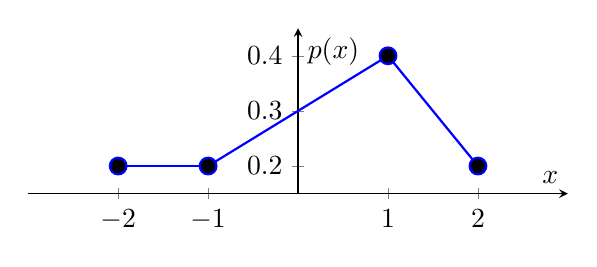
\begin{tikzpicture}
\begin{axis}[
    axis lines=middle,
    xmin=-3, xmax=3,
    ymin=0.15, ymax=0.45,  % Встановіть максимальне значення, відповідно до ваших значень p_i
    xlabel={$x$},
    ylabel={$p(x)$},
    xtick={-2,-1,1,2},
    ytick={0,0.1,0.2,0.3,0.4,0.5},
    yticklabels={0, 0.1, 0.2, 0.3, 0.4, 0.5},
    y=7cm,
]

\addplot[draw=blue, thick, only marks, mark=*, mark size=3pt] table {
x y
-2 0.2
-1 0.2
1 0.4
2 0.2
};

% \addplot[draw=blue, thick] coordinates {(-2, 0) (-2, 0.2)};
\addplot[draw=blue, thick] coordinates {(-2, 0.2) (-1, 0.2)};
\addplot[draw=blue, thick] coordinates {(-1, 0.2) (1, 0.4)};
\addplot[draw=blue, thick] coordinates {(1, 0.4) (2, 0.2)};

\end{axis}
\end{tikzpicture}
	\caption{многокутник розподілу}
\end{figure}

\subparagraph{Математичне сподівання}
$
M = -2*0.2-1*0.2+1*0.4+2*0.2 = 0.2
$
\subparagraph{Дисперсія}
$
	D = 0.2*(-2^2) +0.2*1 +0.4 +0.2*4 - 0.2^2 = 2.16
$
\subparagraph{Квадратичне відхилення}
$
	\sigma = \sqrt{D} = \sqrt{2.16} \approx 1.46969384566990685891
$

\Answer{
	$M = 0.2$,
	$D = 2.16$,
	$\sigma = 1.4697$
}

\Problem{
	Задано функцію розподілу випадкової величини $\xi$:
	$$
		F(x)=
		\begin{cases}
			0, & x \leq 0; \\
			\sin x, & x \in (0; \pi/2]; \\
			1, & x \geq \pi/2.
		\end{cases}
	$$
	Знайти моду, медіану, математичне сподівання
	та дисперсію випадкової величини $\xi$.
}

\subparagraph{Щільність}
$
	f_\xi(x) =
\begin{cases}
	0, x \notin (0, \frac{\pi}{2}) \\
	\cos x, x \in (0, \frac{\pi}{2})
\end{cases}
$

\subparagraph{Мода} $m=0$, оскільки $\cos 0 = 1$ --- найбільше значення функції щільности.
\subparagraph{Медіана} $F(\mu) = \frac{1}{2}$,
$
\sin \mu = \frac{1}{2} \implies \mu = \frac{\pi}{6}
$

\subparagraph{Математичне сподівання}

$$
M_\xi =
\int_0^{\frac{\pi}{2}} x \cos x \,dx
% = \int_0^{\frac{\pi}{2}} x\,d(sin x)
= x\sin x \Big|_0^{\frac{\pi}{2}}
- \int_0^{\frac{\pi}{2}} \sin x\,dx
= \frac{\pi}{2} + \cos x \Big|_0^{\frac{\pi}{2}} = \frac{\pi}{2} - 1
$$

\subparagraph{Дисперсія}

\begin{dmath} % <++>
M_{\xi^2} =
\int_0^{\frac{\pi}{2}} x^2 \cos x \,dx
% = \int_0^{\frac{\pi}{2}} x^2\,d(sin x)
= x^2\sin x \Big|_0^{\frac{\pi}{2}}
- 2\int_0^{\frac{\pi}{2}} x \sin x\,dx
= \frac{\pi^2}{4} + 2
\int_0^{\frac{\pi}{2}} x\,d(\cos x)
%
= \frac{\pi^2}{4} + 2(x\cos x \Big|_0^{\frac{\pi}{2}} -
\int_0^{\frac{\pi}{2}} \cos x \, dx)
= \frac{\pi^2}{4} - 1
\end{dmath}

$$
D_\xi =
M_{\xi^2} -
(M_\xi)^2
= \frac{\pi^2}{4} - 1
- (\frac{\pi}{2} - 1)^2
= \frac{\pi^2}{4} - 1
- \frac{\pi^2}{4} + \pi - 1
= \pi -2
$$

\Answer{
$m=0$,
$\mu = \frac{\pi}{6}$,
$M_\xi = \frac{\pi}{2} - 1$,
$D_\xi = \pi -2$
}

\Problem{
	Випадкова величина $\xi$ задана функцією розподілу:
	$$
		F_{\xi}(x)=
		\begin{cases}
			0, & x \leq 0; \\
			A\ln(x^2+1), & x \in (0; 1]; \\
			1, & x \geq 1.
		\end{cases}
	$$
	Знайти сталу $A$, а також $M_{\eta}$ і $D_{\eta}$, якщо $\eta=\sqrt{\xi}$.
}

\subparagraph{$A$}

Запишемо функцію щільності
	$f_\xi(x) = F'_\xi(x)$
:

\[
	f_\xi(x) =
	\begin{cases}
		0, x \notin (0,1) \\
		\frac{2Ax}{x^2+1}, x \in (0,1)
	\end{cases}
\]

\[
	\int_0^1 \frac{2Ax}{x^2+1} \,dx
	= A\ln(x^2+1) \Big|_0^1
	= A\ln 2 = 1 \implies
	A = \frac{1}{\ln 2}
\]

\subparagraph{Математичне сподівання}

\[
	M_\eta = M_{\sqrt{\xi}} = \int_0^1 \sqrt{x} f_\xi(x)\, dx
	= \frac{1}{\ln 2} \int_0^1 \frac{2x\sqrt{x}}{x^2+1} \, dx
	\implies
	\left[
	\begin{array}{lc}
		\sqrt{x} = t & x = 0 \implies t = 0 \\
		x = t^2 & x = 1 \implies t = 1 \\
		dx = 2t\,dt
	\end{array}
	\right]
\]

\[
	\frac{4}{\ln2} \int_0^1 \frac{t^4}{t^4+1} \, dt
	=
	\frac{4}{\ln2}
	\left(
		\int_0^1 \,dt -\int_0^1\frac{1}{t^4+1} \, dt
	\right)
	=
	\left(
		t \Big|_0^1 -\int_0^1\frac{1}{t^4+1} \, dt
	\right)
\]

\[
	t^4+1 = (x^2-\sqrt{2}+1)(x^2+\sqrt{2}+1) \implies
	\frac{1}{t^4+1} = \frac{B_1x+C_1}{x^2-\sqrt{2}x+1} + \frac{B_2x+C_2}{x^2+\sqrt{2}x+1}
\]
\[
	\frac{1}{t^4+1} = \frac{x^3(B_1+B_2)+x^2(C_1+C_2+\sqrt{2}B_1-\sqrt2B_2) + x(B_1+B_2+\sqrt{2}C_1+\sqrt{2}C_2)+C_1+C_2}
	{(x^2-\sqrt{2}x+1)(x^2+\sqrt{2}x+1)}
\]

\[
	\begin{cases}
		B_1+B_2=0 \\
		C_1+C_2+\sqrt{2}(B_1-B_2)=0 \\
		B_1+B_2+\sqrt{2}(C_1-C_2)=0 \\
		C_1+C_2=1
	\end{cases}
	\implies
	\begin{cases}
		C_1=C_2=\frac{1}{2} \\
		B_1=-\frac{1}{2\sqrt2}, \\
		B_2=\frac{1}{2\sqrt2}
	\end{cases}
\]

\[
	\int \frac{dx}{x^4+1} =
	-\frac{1}{2\sqrt2} \int \frac{x-\sqrt2}{x^2-\sqrt2x+1} \,dx
	+\frac{1}{2\sqrt2} \int \frac{x+\sqrt2}{x^2+\sqrt2x+1} \,dx
\]

\begin{dmath}
	\frac{1}{2\sqrt2} \int \frac{x+\sqrt2}{x^2+\sqrt2x+1} \,dx
	=
	\frac{1}{2\sqrt2}
	*
	\frac{1}{2}
	\left(
	\int \frac{2x+\sqrt2}{x^2+\sqrt2x+1}\,dx \left[ = \ln\left(\left|{x}^{2}+\sqrt{2}\,x+1\right|\right) \right]
	+ \int \frac{\sqrt2}{(x+\frac{1}{\sqrt2})^2+\frac{1}{2}}\,dx
 \left[ =
2\,\arctg\left(\sqrt2 x + 1\right)
\right]
	\right)
\end{dmath}

Так само,

$$
	-\frac{1}{2\sqrt2} \int \frac{x-\sqrt2}{x^2-\sqrt2x+1} \,dx =
	-\frac{1}{4\sqrt2} \left(
	\ln\left({x}^{2}-\sqrt{2}\,x+1\right)-2\,\arctg\left(\sqrt2 x - 1\right)+C
	\right)
	+C
$$

$$
	\int \frac{dx}{x^4+1} =
	\frac{1}{4\sqrt2}
	\ln
	\frac{ {x}^{2}+\sqrt{2}\,x+1 }
	{ {x}^{2}-\sqrt{2}\,x+1 }
	+\frac{1}{2\sqrt2}
	\left(
	\arctg(\sqrt2 x + 1)
	+
	\arctg(\sqrt2 x - 1)
	\right)
	+C
$$

Отже:

\begin{dmath}
	M_\eta
	% \frac{4}{\ln 2}
	% \left(
	% 	1-\int_0^1\frac{dt}{t^4+1}
	% \right)
	=
	\frac{4}{\ln 2}
	-
	\frac{4}{\ln 2}
	\left[
	\frac{1}{4\sqrt2}
	\ln
	\frac{ {t}^{2}+\sqrt{2}\,t+1 }
	{ {t}^{2}-\sqrt{2}\,t+1 }
	+\frac{1}{2\sqrt2}
	\left(
	\arctg(\sqrt2 t + 1)
	+
	\arctg(\sqrt2 t - 1)
	\right)
	\right]
	\Big|_0^1
% =
% 	\frac{4}{\ln 2}
% 	-
% 	\frac{4}{\ln 2}
% 	\left[
% 	\frac{1}{4\sqrt2}
% 	\ln
% 	\frac{ {t}^{2}+\sqrt{2}\,t+1 }
% 	{ {t}^{2}-\sqrt{2}\,t+1 }
% 	+\frac{1}{2\sqrt2}
% 	\left(
% 	\arctg(\sqrt2 t + 1)
% 	+
% 	\arctg(\sqrt2 t - 1)
% 	\right)
% 	\right]
% 	+0
=
	\frac{4}{\ln 2}
	-
	\frac{4}{\ln 2}
	\left[
	\frac{1}{4\sqrt2}
	\ln
	\frac{ 2+\sqrt{2} }
	{ 2-\sqrt{2} }
	+\frac{1}{2\sqrt2}
	\left(
	\arctg(\sqrt2 + 1)
	+
	\arctg(\sqrt2 - 1)
	\right)
	\right]
	+0
	= 0.7676696
\end{dmath}

\begin{minted}{r}
> integrand <- function(x) {2*x*sqrt(x)/(x^2+1)}
> integrate(integrand, 0, 1)
0.532108 with absolute error < 7.9e-06
> 1/log(2) * 0.532108
[1] 0.7676696
\end{minted}

\subparagraph{Дисперсія}

$
D_\eta = \underbrace{M_{\eta^2}}_{\downarrow} - M_{\eta}^2
= 0.61921 - 0.7676696^2 =
0.02989338523584
$

$$
M_{\eta^2} = M_\xi = \int x f_\xi(x)\,dx
= \frac{2}{\ln 2}
\left(
	\int_0^1\,dx - \int_0^1\frac{dx}{x^2+1}
\right)
= \frac{2}{\ln 2}
\left(
	x \big|_0^1 - \arctg x\big|_0^1
\right)
= \frac{2}{\ln 2}
\left(
	1 - \frac{\pi}{4}
\right)
% = 0.61921
$$

\Answer{
	$A = \frac{1}{\ln 2},
	M_\eta = 0.7676,
	D_\eta = 0.0298
	$
}

% \Problem{
% 	Знайти характеристичну функцію для випадкової величини $\xi$, заданої законом розподілу
% \\
% 	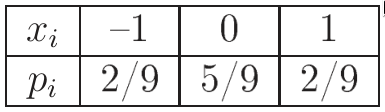
\includegraphics[width=.2\textwidth]{table1}
% \\
% 	і за знайденою характеристичною функцією знайти $M_\xi$ та $D_\xi$
% }
% \Answer{<++>}

% \Problem{
% }
% \Problem{
% }
% \Problem{
% }

\end{document}
